\chapter{The Robot Software System (ROS)}

The ROS system is designed to contain as few customizations as possible. This allows our team and future teams to take advantage of as many pre-existing ROS packages as possible. Note that this section of the report assumes familiarity with ROS, basic ROS functionality, catkin and how to create and use ROS packages.

\section{Preparing to Run the ROS Stack and Setting up the Repository}

The NUC onboard the Gator already has all the packages required to run the software stack in ROS Indigo. However, if you want to run the software stack on another computer, you should try to use ROS Indigo unless the IV Lab has upgraded its fleet. You'll then need the following 3rd-party ROS packages to be installed using apt-get and the package manager (e.g. sudo apt-get install ros-indigo-robot-localization):

\begin{enumerate}
\item Robot Localization: \url{http://wiki.ros.org/robot \textunderscore localization}
\item move base: \url{http://wiki.ros.org/move \textunderscore base}
\item URDF: \url{http://wiki.ros.org/urdf}
\item Robot State Publisher: \url{http://wiki.ros.org/robot\textunderscore state\textunderscore publisher}
\item DWA Local Planner: \url{http://wiki.ros.org/dwahttp://wiki.ros.org/dwa_local_planner localhttp://wiki.ros.org/dwa_local_planner planner}
\end{enumerate}

\noindent Once these packages are installed, you can then download the Gator repository from here: \url{https://github.com/olinrobotics/GatorResearch}. Once downloaded, change directory into the master \textunderscore ws folder and then run the command "catkin \textunderscore make". Once done, run the command "source devel/setup.bash". If desired, you should add this sourcing step to your bashrc file so that you don't have to do this manually every time you open a new terminal.

\newpage

\section{ROS Navigation Overview}

The following diagram shows how the ROS Navigation Stack is designed to be used:

\begin{figure}[h!]
\centering
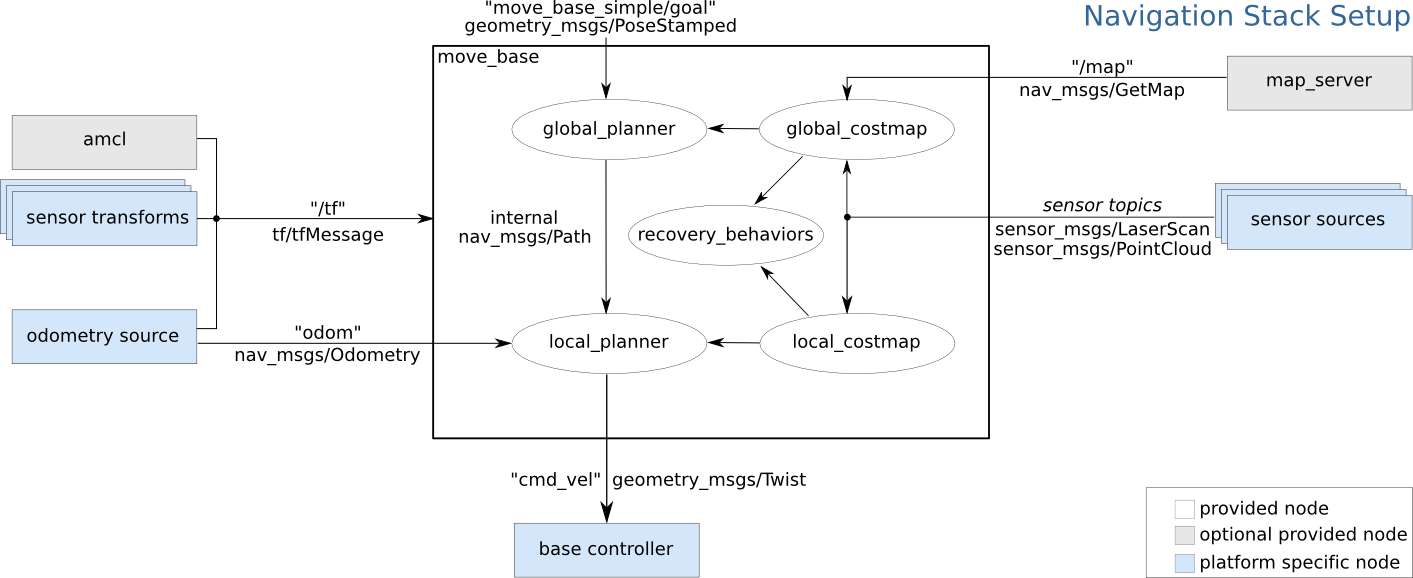
\includegraphics[scale=.35]{Photos/rosnavoverview.png}
\caption{Overview of the Setup of the ROS Navigation Stack}
\label{fig:rosnavoverview}
\end{figure} 

\noindent As can be seen in Figure \ref{fig:rosnavoverview}, the ROS Navigation Stack is made up of a core (move\textunderscore base) and several supporting packages (transforms, odometry sources, a map server, sensor sources and a base controller). 

\subsection{move\textunderscore base (controller)}

The core of the ROS Navigation Stack is the move\textunderscore base package (the big box in the center of Figure \ref{fig:rosnavoverview} that is installed using the package manager. The move\textunderscore base package is responsible for all operations involving commanding the base to move. As shown in Figure \ref{fig:rosnavoverview}, there are 5 key elements to the move\textunderscore base package:

\begin{enumerate}
\item global\textunderscore planner: The global planner is responsible for planning a path to get from where the vehicle is to its destination, regardless of the distance between the origin and the destination. There are several standard options for global planners that can be used as a global planner and any global planner can be used as long as it adheres to the nav\textunderscore core::BaseGlobalPlanner C++ interface defined in the nav\textunderscore core package.
\item global\textunderscore costmap: The global costmap is responsible for maintaining an understanding of all known fixed obstacles in the world of the vehicle using a concept known as cost. For every move the vehicle makes, there is an associated cost to get there. If there are no obstructions to the vehicle, the cost is relatively low. However, if there are obstacles such as tree stumps or rocks at a location, then the cost to be in that location increases. When the vehicle is planning a global path to get from where it is to where it is going to be, the global planner will try to find a route that minimizes the cost to the vehicle of getting from origin to destination. Note that obstacles and features in the global costmap are not updated in real-time. The global costmap is simply created and set beforehand and referenced during normal operation. 
\item local\textunderscore planner: The local planner, like the global planner, is responsible for path planning. However, the local planner is responsible for path planning at a smaller distance scale to plan new paths around obstacles and other obstructions in real-time. So, the local planner is used to plan paths in the immediate vicinity of the vehicle's current position unlike the global planner that can be used to plan paths over much longer distances. 
\item local\textunderscore costmap: The local costmap, like the global costmap, is responsible for maintaining an understanding of all known obstacles in the world of the vehicle using the concept of cost. However, the key difference between the local and global costmaps is that the local costmap is updated in real-time using LiDAR data from the vehicle unlike the global costmap that remains static during operation. Using the LiDAR data from the vehicle, detected obstacles are added to the local costmap and the vehicle will then use the local costmap to plan a path around the obstacle.
\item recover\textunderscore behaviors: Recovery behaviors are used to help the vehicle recover from path planning errors that might be due to erroneous data or a field of view that is too narrow to see a possible path. However, the standard recover behaviors in ROS were written for a holonomic robot that uses differential drive and can therefore turn in place. Since the John Deere Gator XUV is Ackermann-steered and therefore cannot turn in place, we simply turn these recovery behaviors off.
\end{enumerate}

\subsection{Transforms (Input)}

Transforms are a key component of any robot and they provide information about where things are relative to other things. Ultimately, a chain of transforms should provide all the information necessary to determine the position and orientation of something on the robot relative to the vehicle's coordinate system. In ROS, these transforms are an input to the navigation stack and typically indicate the position and orientation of sensors and other key components in relation to other sensors or key components. For example, a transform would indicate the location and orientation of the LiDARs relative to the origin of the vehicle coordinate system. These transforms are important because sensor data is only useful when it can used in conjuction with other systems. However, to work with other systems all these sensors and systems need to be operating with respect to some reference point and, more importantly, they need to be operating with respect to THE SAME refrence point. So, transforms can help transform sensor data from being with reference to the sensor's own local coordinate system to being with reference to the vehicle coordinate system, which is the coordinate system used by all sensors and systems on the John Deere Gator XUV.\\ \\
%
There are 2 important types of transforms:

\begin{enumerate}
\item Sensor Transforms: these are transforms that indicate the position and orientation of the sensor relative to some reference point. The sensor transforms on the John Deere Gator XUV will be discussed in more detail later.
\item Robot Joint Transforms: these are transforms that indicate the position and orientation of all joints between the different parts of the robot and also indicate what type of joints they are (e.g. fixed, revolute). 
\end{enumerate} 

\noindent Regardless of what type of transform it is, all transforms are written in a file known as a Univeral robot Definition File (URDF). Based on the information in that file, the transforms are published by a package known as "Robot State Publisher", which reads the URDF file and then publishes the numerican value of the transforms. More details on this can be found later in this document.

\subsection{Odometry Sources (Input)}
\label{sec:gatorloc}

Odometry sources are another key input to the ROS Navigation Stack. Unlike transforms, odometry sources provide information about the location of the origin of the vehicle's coordinate system (which moves with the vehicle when the vehicle moves) relative to some fixed (inertial) reference frame that does not move even when the vehicle is moving. Common sources of odometry include wheel odometry for dead reckoning as well as GPS for getting absolute, geospatial information about where the vehicle is.\ \\
%
There are three fixed reference frames used by the John Deere vehicle for navigating:

\begin{enumerate}
\item The Odom Frame: the odom frame is a fixed frame that is typically used as the fixed reference frame for the location of the vehicle during deadreckoning. As such, information provided with reference to the odom frame provides information about the location of the vehicle relative to where it was when the navigation stack was first run. Sensors that contribute to the location of the robot with reference to the odom frame usually provide continuous, uninterrupted streams of data (e.g. IMU and wheel velocity from wheel encoders)
\item The Map Frame: the map frame is a fixed frame that is typically used as the fixed reference frame for location of the vehicle when the vehicle is travelling within a mapped or known environment. If the vehicle starts at the origin of the map, then the odom and map frames will be on top of each other. Otherwise, the origin of the map frame will be wherever the origin of the map was defined during mapping. Sensors that contribute to the location of the robot with referene to the map frame are usually more prone to dropouts (e.g. GPS)
\item The UTM Frame: the origin of the UTM frame is the origin of all GPS coordinates. Thus, information provided with reference to the UTM frame indicates the GPS position of the vehicle
\end{enumerate}

\noindent The vehicle can be localized using any number of sensor sources and, in some cases, having multiple sensors contributing to vehicle localization can help reduce the error in the vehicle's location information. However, using multiple sensor sources requires the ability to fuse those sensor sources to ultimately generate one source of information about the location of the vehicle. So, the John Deere vehicle uses the robot\textunderscore localization package that provides pre-written nodes for fusing sensor sources to obtain odometry information. The robot\textunderscore localization package provides three nodes for obtaining odometry information:

\begin{enumerate}
\item ekf\textunderscore localization\textunderscore node: The EKF localization node uses an Extended Kalman Filter (EKF) to fuse sensor data. On the John Deere vehicle, two copies of this node are run: 
\begin{enumerate}
\item One copy is used to fuse all continuous sources of sensor information: IMU and wheel odometry. The output is the transform from the vehicle's coordinate system (origin on the ground under the rear axle of the vehicle) to the odom frame (wherever the vehicle was when the navigation stack was first run). 
\item Another copy is used to fuse the above odom frame information with GPS information that is susceptible to drop-outs. The output is a transform from the vehicle's coordinate system (origin on the ground under the rear axle of the vehicle) to the map frame.
\end{enumerate}
\item ukf\textunderscore localization\textunderscore node: this node is similar to the ekf\textunderscore localization\textunderscore node except that it uses a slightly different Kalman filter. This node is not used at all on the John Deere Vehicle.
\item navsat\textunderscore transform\textunderscore node: this node uses the raw GPS information as well as IMU information to create a transform between the vehicle's coordinate system to the UTM frame. 
\end{enumerate}

\subsection{Map Server}

The map server is exactly what it sounds like: it is a server that stores a copy of the map that the vehicle should be driving in. Typically, when the vehicle is first powered up, a human operator would need to tell the robot where in the map it started. The robot will then take care of keepign itself localized within that map while driving. Typically, the map is generated using the gmapping package or any other ROS mapping package. On the John Deere vehicle, this has not been implemented at the time of writing.

\subsection{Sensor Sources}

Sensor sources are very important to the vehicle for localization (as discussed above) as well as position confirmation and obstacle avoidance. Data such as IMU, GPS and wheel velocity information are used for localization while LiDAR data is used for obstacle avoidance and to confirm that the majority of the obstacles and features detected by the LiDAR are also features that can be found in the map.

\subsection{Base Controller}

The base controller is also exactly what it sounds like: it is a node that knows how to control the base given the desired heading and velocity commands (also known as cmd\textunderscore vel commands) that the Navigation Stack will produce. On the John Deere vehicle, the entire LabVIEW code serves as the vehicle controller. 

\section{Custom Catkin Packages}

In addition to the standard packages discussed above, the John Deere vehicle also has several custom packages that the team wrote to allow the vehicle to make use of the ROS navigation stack.  These include:

\begin{enumerate}
\item gator\textunderscore odom: Contains a script and launch file that generates the wheel odometry information
\item gator\textunderscore nav: Contains the launch and yaml files that are required to set the settings for the navigation stacks and launch the navigation stack
\item gator\textunderscore msgs: Defines any custom messages that are created specifically for the Gator
\item gator\textunderscore localization: Contains the launch files needed to launch the necessary robot\textunderscore localization and navsat\textunderscore transform nodes to allow the Gator to localize accurately
\item gator\textunderscore description: Contains the launch files, STL files and URDF file that create a visual model of the Gator
\item gator\textunderscore communication: Contains python scripts that listen to all sensor data coming from LabVIEW over UDP and publishes it in ROS to the appropriately named topic
\item gator: An unused package that was set up for the purpose of containing all the highest-level launch files for running the vehicle
\end{enumerate}

Each of these packages will be discussed in more detail in the sections below.

\subsection{gator\textunderscore odom}

The gator\textunderscore odom package contains the following files:

\begin{enumerate}
\item wheel\textunderscore odom.py: Creates a wheel odometry node that reads the odometry calculations made by LabVIEW and uses that odometry information to compute the odometry transform from the origin of the vehicle (i.e. on the ground under the rear axle of the vehicle) to the odom frame.
\item wheel\textunderscore odom.launch: The launch file that launches wheel\textunderscore odom.py as a node in ROS to calculate and provide the odom frame transform. It also specifies the vehicle\textunderscore length parameter that wheel\textunderscore odom.py needs to calculate the odom frame transform.
\end{enumerate}

\subsection{gator\textunderscore nav}

The gator\textunderscore nav package provides all the files needed to setup and run the navigation stack. Since the navigation stack uses standard ROS packages, the gator\textunderscore nav package provides the following parameter files to set the right settings for the standard ROS navigation stack:

\begin{enumerate}
\item costmap \textunderscore common\textunderscore params.yaml: A text file that sets the required parameters that are common to both the local and global costmaps. Full details can be found here: \url{http://wiki.ros.org/navigation/Tutorials/RobotSetup}  in the Costmap Configuration section.
\item global\textunderscore costmap\textunderscore params.yaml: A text file that sets the required parameters specific to the global costmap. Full details can be found at the same URL as the URL provided in bullet point 1.
\item local\textunderscore costmap\textunderscore params.yaml: A text file that sets the required parameters specific to the local costmap. Full details can be found at the same URL as the URL provided in bullet point 1.
\item dwa\textunderscore local\textunderscore planner\textunderscore params.yaml: A text file that sets the parameters for the DWA local planner used on the John Deere vehicle. Full details on the parameters required can be found at: \url{http://wiki.ros.org/dwa\textunderscore local\textunderscore planner#Parameters}.
\item global\textunderscore planner\textunderscore params.yaml: A text file that sets the parameters for the global\textunderscore planner package used as the global planner on the John Deere vehicle. Full details on the required parameters can be found at: \url{http://wiki.ros.org/global\textunderscore planner?distro=jade#Parameters}
\end{enumerate}

In addition, the gator\textunderscore nav package provides the following launch files:

\begin{enumerate}
\item move\textunderscore base.launch: A launch file that launches the standard ROS navigation stack with the parameters provided above. Full details can be found at: \url{http://wiki.ros.org/navigation/Tutorials/RobotSetup#Creating\textunderscore a\textunderscore Launch\textunderscore File\textunderscore for\textunderscore the\textunderscore Navigation\textunderscore Stack}
\item gator\textunderscore config.launch: A launch file that launches the vehicles configuration files including launching all sensors, launching all localization nodes, the state publisher and the wheel odometry publisher. Full details can be found at: \url{http://wiki.ros.org/navigation/Tutorials/RobotSetup#Creating\textunderscore a\textunderscore Robot\textunderscore Configuration\textunderscore Launch\textunderscore File}
\item navigation.launch: A launch file that launches the first 2 launch files together to properly launch the entire navigation stack and required components.
\end{enumerate}

\subsection{gator\textunderscore msgs}

This package simply provides definitions for custom messages used on the vehicle. The only two provided at the time of writing are a Drive State message and a GlobalPose message.

\subsection{gator\textunderscore localization}

This package provides all the localization nodes required for the vehicle. Since the vehicle's localization is carried out by the robot\textunderscore localization package, this package merely provides launch files that does the actual launching. An explaination for the high-level organization of the localization package was discussed earlier in Section \ref{sec:gatorloc}.\\ \\
%
Full details on the parameters speified in the launch file can be found at: \url{http://wiki.ros.org/robot_localization}\\ \\
%
The launch files included are:

\begin{enumerate}
\item ekf\textunderscore loc\textunderscore cont.launch: A launch file that launches a copy of the EKF localization node for handling the continuous data coming from the IMU and wheel odometry. The output is a transform from the vehicle coordinate system to the odom frame.
\item ekf\textunderscore loc\textunderscore gps.launch: A launch file that launches a second copy of the EKF localization node for fusing the output of the continuous data localization node with the GPS data. The output is a transform from the odom to the map frame.
\item navsat\textunderscore transform.launch: A launch file that launches the navsat transform node that filters the raw GPS data
\item localization.launch: A launch file that launches all 3 launch files above to properly launch a complete localization package.
\end{enumerate}

\subsection{gator\textunderscore description}

The gator\textunderscore description package provides all the required information for describing the vehicle, its sensors and other hardware as well as where these items are located on the vehicle. The package provides the following files:

\begin{enumerate}
\item BaseGator.urdf: A URDF file that describes how to assemble a model of the vehicle using the different parts
\item STL Files: STL files for all the different parts of the vehicle that are needed to assemble a full model of it. The STL files include:
\begin{enumerate}
\item The base vehicle
\item Front camera mouting assembly
\item Front peg board
\item Left and right tilt unit
\item left and right LiDAR
\end{enumerate}
\item display.launch: A launch file that launches the robot\textunderscore description package to parse the URDF. The launch file also launches the joint state publisher and robot state publisher that publish the joint and robot states. Finally, the launch file also launches rviz to visualize the vehicle model.
\item gator\textunderscore state\textunderscore pub.launch: A launch file that is exactly the same as the display.launch file, but without the additional rviz launching step. This file is used by the gator\textunderscore nav package to launch the localization elements of the code without also launching rviz.
\end{enumerate}

\subsection{gator\textunderscore communication}

The gator\textunderscore communication package is a large package that provides all the required elements for the ROS code to communicate with the LabVIEW code over UDP. In the package, there are 5 files:

\begin{enumerate}
\item The "launch" file contains:
\begin{enumerate}
\item sensors.launch: A launch file that launches all the nodes to read all the data being transmitted by LabVIEW
\item teleop\textunderscore key.launch: A launch file that launches the nodes required to teleoperate the vehicle via keyboard
\end{enumerate}
\item The "msg" file contains message definitions that are no longer in use but could be used in the future if required.
\item The "scripts" file contains all the scripts that are needed to listen over UDP for the data coming from LabVIEW and re-publish them in ROS on the appropriate topic.
\item The "src" and "srv" files contain example ROS publisher and subscriber files and ROS service definition files respectively. They are not used directly on the vehicle but can be used as templates to create publishers or subscribers or to create a ROS service if needed.
\end{enumerate}

\noindent It is worth noting that this document will not discus full details of each of the scripts that transfers data from LabVIEW to ROS. Full documentation can be found within the scripts themselves.

\subsection{gator}

The gator package was created with the intention of storing high-level launch files that launch the entire vehicle's packages at once. At the time of writing, however, the team did not manage to get these packages written and so this package remains blank for a future team to complete it.